\documentclass[9pt,twocolumn,twoside]{gsajnl_modified}
% Use the documentclass option 'lineno' to view line numbers

\usepackage[htt]{hyphenat}  % https://tex.stackexchange.com/a/543
\usepackage[export]{adjustbox}
\usepackage{xurl}
\usepackage{stfloats}
\usepackage[leftcaption]{sidecap}
\sidecaptionvpos{figure}{t}

\renewcommand{\topfraction}{0.9}	% max fraction of floats at top
    \renewcommand{\bottomfraction}{0.8}	% max fraction of floats at bottom
    %   Parameters for TEXT pages (not float pages):
    \setcounter{topnumber}{2}
    \setcounter{bottomnumber}{2}
    \setcounter{totalnumber}{4}     % 2 may work better
    \setcounter{dbltopnumber}{2}    % for 2-column pages
    \renewcommand{\dbltopfraction}{0.9}	% fit big float above 2-col. text
    \renewcommand{\textfraction}{0.07}	% allow minimal text w. figs
    %   Parameters for FLOAT pages (not text pages):
    \renewcommand{\floatpagefraction}{0.7}	% require fuller float pages
	% N.B.: floatpagefraction MUST be less than topfraction !!
    \renewcommand{\dblfloatpagefraction}{0.7}	% require fuller float pages

\newcommand\jdbcomment[1]{\textcolor{red}{[#1]}}
\newcommand\rancomment[1]{\textcolor{blue}{[#1]}}

\title{Estimated fitness effects of amino-acid mutations to SARS-CoV-2 proteins}

\author[*]{\Large Jesse D. Bloom$^{1,2,3^*}$ and Richard A. Neher$^{4,5}$}

\affil[1]{Basic Sciences and Computational Biology, Fred Hutchinson Cancer Center

}
\affil[2]{Department of Genome Sciences, University of Washington

}
\affil[3]{Howard Hughes Medical Institute

}
\affil[4]{Biozentrum, University of Basel

}
\affil[5]{Swiss Institute of Bioinformatics

\jdbcomment{Should we add Angie Hinrichs as co-author? She helped answer some UShER questions on GitHub. Probably just acknowledgments is fine, but what do you think?}

}

\keywords{}

\runningtitle{} % For use in the footer
\runningauthor{}

\begin{abstract}
Knowledge of the fitness effects of mutations to SARS-CoV-2 can inform risk assessment of new viral variants and targeting of therapeutics to constrained sites where resistance is unlikely to emerge.
However, experimentally determining the effects of mutations is challenging: we lack tractable lab assays for the functions of many SARS-CoV-2 proteins, and for this reason systematic deep mutational scanning has been applied to only two of the virus's proteins.
Here we develop a new approach that leverages millions of publicly available SARS-CoV-2 sequences to estimate the effects of most amino-acid mutations accessible by single-nucleotide changes.
To do this, we first calculate how many independent times each mutation is expected to occur along the SARS-CoV-2 phylogeny in the absence of selection.
We then compare these expected counts to the actual observed counts of each mutation, and use the ratio of counts to estimate the effect of each mutation.
For the two proteins with deep mutational scanning data, our sequence-based estimates correlate with experimental measurements nearly as well as independent experiments correlate with each other.
For most genes, synonymous mutations are nearly neutral, stop-codon mutations are deleterious, and amino-acid mutations have a range of effects.
However, some viral accessory proteins are under little to no selection during SARS-CoV-2 evolution in humans.
We provide interactive visualizations of the estimated effects of individual mutations to each viral protein, enabling these data to be easily used in viral surveillance and drug development.
Overall, our work provides a framework to estimate the effects of mutations to any virus (or organism) for which the number of available sequences is sufficiently large that that each neutral mutation independently occurs many times.
\end{abstract}

\begin{document}

\maketitle
\thispagestyle{firststyle}
%\marginmark
\firstpagefootnote

\correspondingauthoraffiliation{}{*\href{mailto:jbloom@fredhutch.org}{jbloom@fredhutch.org} or \href{mailto:richard.neher@unibas.ch}{richard.neher@unibas.ch}}
\vspace{-33pt}% Only used for adjusting extra space in the left column of the first page

\lettrine[lines=2]{\color{color2}B}{}ackground. It's important to understand effects of individual mutations.

Experiments have filled this role for some viral proteins (spike, Mpro), but not for majority of SARS-CoV-2 viral protein.

An alternative is sequence-based estimates, which so far have focused largely on clade growth and identification of mutations that mediate immune escape or increase transmissibility \citep{obermeyer2022analysis,lee2022inferring}.
Mutations that are repeatedly observed at the base of clades that grow faster than the background likely contribute to growth.
Such adaptive mutations are only a small minority of all available mutations and which mutations are adaptive depends on the environment (immunity) and the genetic background.
The great majority of mutations, however, have either small fitness effects (approximately neutral) or are deleterious to viral replication.
Here, we describe an approach to quantify the fitness cost of these mutations based on comparing expected versus observed counts.

\rancomment{older paper on flu where not counts but trajectories were used to partition sequences into good and bad \citep{strelkowa2021clonal}}

\section{Results}

\subsection{Theory}
\jdbcomment{Include Richard's calculations, either in entirety or summarized with details in Methods / Appendix}

\begin{figure*}
{\bf \Large A \hspace{0.47\linewidth} B}

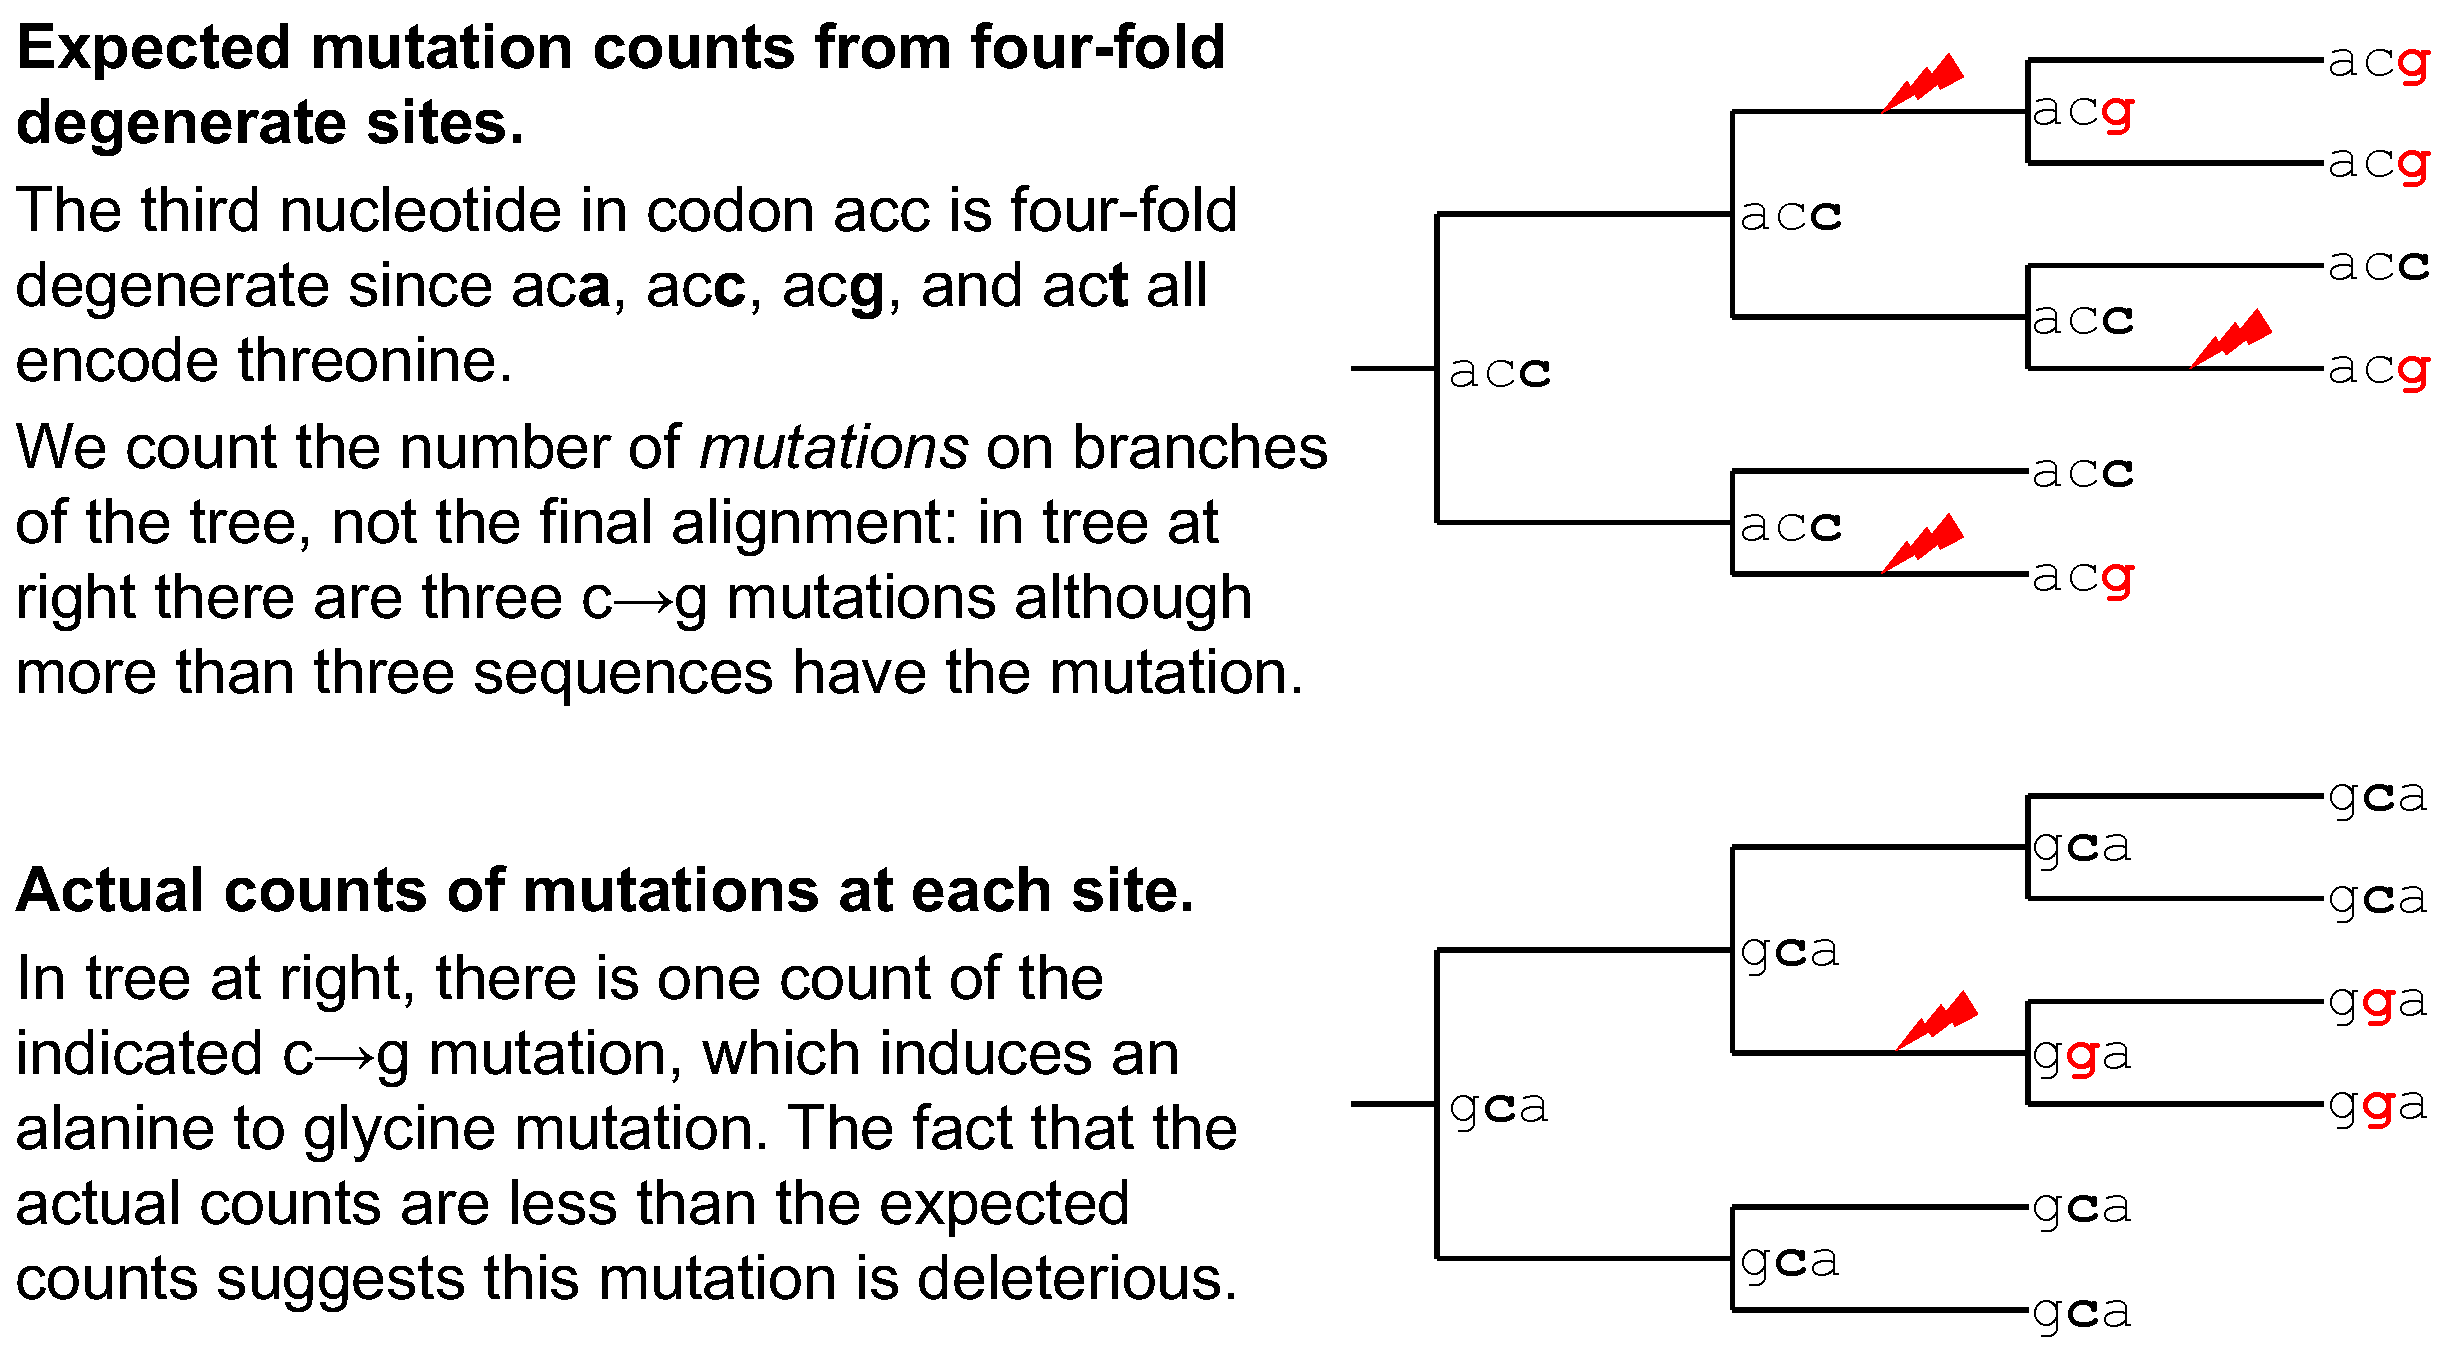
\includegraphics[width=0.48\linewidth,valign=t]{figs/schematic/schematic.pdf}
\hspace{0.02\linewidth}
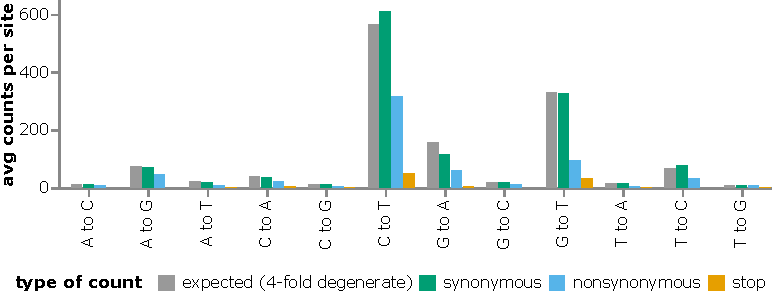
\includegraphics[width=0.5\linewidth,valign=t]{figs/avg_counts.pdf}
\caption{
Calculation of expected versus actual counts for each mutation.
{\bf (A)}
The number of expected counts of each type of nucleotide mutation is computed from the observed counts at four-fold degenerate sites,
and then compared the actual observed counts of each mutation.
Note that the counts represent independent occurrences of each mutation on the tree, not counts of mutations in the alignment of observed sequences (a single occurrence of a mutation can be present in many sequences in an alignment).
{\bf (B)}
Expected versus actual counts for each nucleotide mutation type averaged across all sites where the mutation is four-fold degenerate, synonymous (including four-fold degenerate), nonsynonymous, or introduces a stop codon.
Synonymous mutations are often roughly neutral, so the number of expected and actual counts are similar, but nonsynonymous and especially stop-codon mutations are often deleterious, so the number of actual counts is generally less than the number of expected counts.
Note that due to the highly uneven mutation spectrum of SARS-CoV-2, some nucleotide mutation types are expected to occur far more often than others.
An interactive version of panel B is at \url{https://jbloomlab.github.io/SARS2-mut-fitness/avg_counts.html}.
\label{fig:expected_vs_actual}
}
\end{figure*}

\begin{figure*}
{\bf \Large A}

\includegraphics[width=\linewidth, trim={0in 0.7in 0 0.05in}, clip=true]{figs/effects_histogram.pdf}

{\bf \Large B}

\includegraphics[width=\linewidth, trim={0in 0.36in 0 0in}, clip=true]{figs/effects_dist.pdf}
\caption{
Distribution of effects of different types of mutations.
{\bf (A)}
Histograms of effects of synonymous, nonsynonymous, and stop-codon mutations across all viral genes.
Neutral mutations have effects of zero, and deleterious mutations have negative effects.
\jdbcomment{Maybe add dotted vertical line at zero to denote neutrality?}
{\bf (B)}
Distribution of effects of each type of mutation for each viral gene.
The dark squares indicate the median effect of mutations of that type for that gene, and the lighter rectangles span the interquartile range.
Mutation types are color-coded as in panel A.
Both panels show only mutations with expected counts of at least 20.
For interactive versions of these plots that allow adjustment of the expected-count cutoff and other options (such as separate histograms for each gene), see \url{https://jbloomlab.github.io/SARS2-mut-fitness/effects_histogram.html} and \url{https://jbloomlab.github.io/SARS2-mut-fitness/effects_dist.html}.
\label{fig:effects_dist}
}
\end{figure*}

\begin{figure*}
\centering
{\bf \Large A \hspace{0.32\linewidth} B \hspace{0.32\linewidth}}

\includegraphics[width=0.32\linewidth]{figs/clade_corr_chart.pdf}
\hspace{0.05\linewidth}
\includegraphics[width=0.32\linewidth]{figs/subset_corr_chart.pdf}
\caption{
Correlations between amino-acid fitness estimates made using different sequence subsets.
{\bf (A)} Estimates made using only sequences from the Omicron BA.2 clade or only the Alpha clade, or {\bf (B)} estimates made using only sequences from the USA or England.
In the scatter plots, each point is a different amino-acid mutation, and the orange text at upper left shows the number of mutations and Pearson correlation coefficient.
Both panels show only mutations with expected counts of at least 20.
For interactive versions of these plots that show correlations among estimates from all clade pairs, allow adjustment of the expected-count cutoff, and allow examination of correlations for just specific genes, see \url{https://jbloomlab.github.io/SARS2-mut-fitness/clade_corr_chart.html} and \url{https://jbloomlab.github.io/SARS2-mut-fitness/subset_corr_chart.html}.
\label{fig:corr}
}
\end{figure*}

\begin{figure*}
{\bf \Large A}

\includegraphics[width=0.9\linewidth]{figs/dms_S_corr.pdf}
\vspace{0.05in}

{\bf \Large B}

\includegraphics[width=0.9\linewidth]{figs/dms_nsp5_corr.pdf}
\caption{
Correlation of fitness effect estimates with experimental measurements from deep mutational scanning studies for {\bf (A)} spike and {\bf (B)} Mpro (nsp5).
Each point is an amino-acid mutation, and the oragne text in the upper left shows the number of mutations and Pearson correlation coefficient.
Data are taken from two independent deep mutational scanning studies for spike~\citep{cite}, and two studies for Mpro~\citep{cite}.
Each sub-panel shows a different set of mutations (those that are measured in each of the two datasets being correlated), and uses a minimum expected count cutoff of 20.
Interactive versions of these plots that enable subsetting on just mutations shown across all datasets and adjustment of the minimum expected count cutoff are at \url{https://jbloomlab.github.io/SARS2-mut-fitness/dms_S_corr.html} and \url{https://jbloomlab.github.io/SARS2-mut-fitness/dms_nsp5_corr.html}.
\label{fig:dms_corr}
}
\end{figure*}

\begin{figure*}
{\bf \Large A}

E protein mutation effects with minimum expected counts of 20 and \textbf{x} marking wildtype identity in Wuhan-Hu-1.

\includegraphics[width=\linewidth, trim={0 0 0 0.4in}, clip=true]{figs/E_view1.pdf}

{\bf \Large B}

E protein mutation effects with minimum expected counts of 5 and \textbf{x} marking wildtype identity in BQ.1.

\includegraphics[width=\linewidth, trim={0 0 0 0.4in}, clip=true]{figs/E_view2.pdf}
\caption{
Effects of amino-acid mutations to E protein.
{\bf (A)} and {\bf (B)} provide two views of the estimated mutation effects with different thresholds for the minimum expected counts and different references used to mark the ``wildtype'' identity, as indicated in the titles above the plots.
For both panels, the area plot at top shows the average effects of mutations at each site, and the heatmap shows the effects of specific amino acids.
An interactive version of this plot at \url{https://jbloomlab.github.io/SARS2-mut-fitness/E.html} enables zooming, mouseovers, and exploration of the data.
Comparable interactive plots for all other viral proteins are linked at \jdbcomment{create landing pad page with these links}.
\label{fig:E}
}
\end{figure*}

\begin{figure*}
{\bf \Large A}

\includegraphics[width=0.8\linewidth]{figs/clade_fixed_muts_hist.pdf}
\vspace{0.05in}

{\bf \Large B}

\includegraphics[width=\linewidth]{figs/clade_fixed_muts.pdf}

\caption{
Effects of amino-acid mutations that have fixed in at least one SARS-CoV-2 clade.
{\bf (A)}
Distribution of fitness effects of all amino-acid mutations relative to Wuhan-Hu-1 and all mutations that are fixed in at least one of the clades (as defined by Nextclade\jdbcomment{cite}).
\jdbcomment{add vertical line at zero to these plots.}
{\bf (B)}
Effects of individual fixed mutations faceted by whether they are in spike or another protein.
Plots show estimates of effects of mutations made across all clades (including those that have fixed the mutation) and just from direct forward occurrences of the mutation in clades in which it has not yet fixed.
Estimates are only shown for mutations with expected counts of at least 20.
Interactive versions of this plot that enable easier exploration of the data are at \url{https://jbloomlab.github.io/SARS2-mut-fitness/clade_fixed_muts_hist.html} and \url{https://jbloomlab.github.io/SARS2-mut-fitness/clade_fixed_muts.html}.
\label{fig:fixed}
}
\end{figure*}

\begin{figure*}
\includegraphics[width=0.8\linewidth, trim={0 1.1in 0 0in}, clip=true]{figs/fitness_vs_terminal.pdf}
\caption{
Relationship between fitness effects of mutations and ratio of counts on terminal (tip) branches versus non-terminal (internal) branches.
Each point is an amino-acid mutation, and the orange text in the upper right give the number of mutations and the Pearson correlation coefficient.
This plot shows only mutations with at least 20 expected counts and 5 actual counts.
An interactive version of this plot that allows filtering by the number of actual or expected counts, or by gene, is at \url{https://jbloomlab.github.io/SARS2-mut-fitness/fitness_vs_terminal.html}.
\jdbcomment{add same color coding as in other panels for synonymous, nonsynonymous, stop types}
\label{fig:terminal}
}
\end{figure*}

\section{Discussion}


{\small

\section{Methods}
\subsection{Code and data availability}
Code and data are at \url{https://github.com/jbloomlab/SARS2-mut-fitness}.

\section{Acknowledgments}
We thank Angie Hinrichs for assistance with resolving several questions related to use of the UShER package and its pre-built mutation-annotated tree \jdbcomment{if we don't add as co-author}.
\jdbcomment{Jesse to acknowledge AVIDD, CEIRR, and R01 grants.}
JDB is an Investigator of the Howard Hughes Medical Institute.

\section{Competing interests}
JDB is on the scientific advisory boards of Apriori Bio, Aerium Therapeutics, Invivyd, the Vaccine Company, and Oncorus.
JDB receives payments as an inventor on a Fred Hutch licensed patents related to deep mutational scanning of viral proteins.

\bibliography{references}
}


\end{document}
